\documentclass[10pt,a4paper]{report}
\usepackage[utf8]{inputenc}
\usepackage[spanish]{babel}
\usepackage{amsmath}
\usepackage{amsfonts}
\usepackage{amssymb}
\usepackage{steinmetz}
\usepackage{circuitikz}
\usepackage{halloweenmath}
\usepackage[normalem]{ulem}
%\usepackage{steinmetz}
%\usepackage[american,siunitx]{circuitikz}
\usetikzlibrary{arrows,shapes,calc,positioning}
%%%%%%%%%%%%%%%%%%%%%%%%%%%%%%%%%%%%%%%%%%%%%%%%
\usepackage{listings}
\usepackage{xcolor}

\definecolor{codegreen}{rgb}{0,0.6,0}
\definecolor{codegray}{rgb}{0.5,0.5,0.5}
\definecolor{codepurple}{rgb}{0.58,0,0.82}
\definecolor{backcolour}{rgb}{0.95,0.95,0.92}

\lstdefinestyle{mystyle}{
	backgroundcolor=\color{backcolour},   
	commentstyle=\color{codegreen},
	keywordstyle=\color{magenta},
	numberstyle=\tiny\color{codegray},
	stringstyle=\color{codepurple},
	basicstyle=\ttfamily\footnotesize,
	breakatwhitespace=false,         
	breaklines=true,                 
	captionpos=b,                    
	keepspaces=true,                 
	numbers=left,                    
	numbersep=5pt,                  
	showspaces=false,                
	showstringspaces=false,
	showtabs=false,                  
	tabsize=2
}
\lstset{style=mystyle}
%%%%%%%%%%%%%%%%%%%%%%%%%%%%%%%%%%%%%%%%%%%%%%%%
\usepackage{graphicx}
\usepackage{multirow}
\usepackage[hyperindex=true,breaklinks=true,colorlinks=true,linkcolor=blue]{hyperref}
\usepackage{multimedia}
\usepackage{subcaption}
\addto\captionsspanish{
\renewcommand{\tablename}{Tabla}
\renewcommand{\listtablename}{\'Indice de Tablas}
}

\usepackage{makeidx}
\usepackage[left=2cm,right=2cm,top=2cm,bottom=2cm]{geometry}
\title{

\includegraphics[scale=0.15]{ucm2.eps} Universidad Complutense de Madrid\\
------------------------------------------------------------------------------------\\
Documentación del software desarrollado para la práctica de control de un motor de cc}
\author{Juan Jiménez}
\graphicspath{{./FIGURAS/}}
\newcommand{\mymotor}[2] % #1 = name , #2 = rotation angle
{\draw[thick,rotate=#2] (#1) circle (10pt)
 node[]{$\mathsf M$} 
++(-12pt,3pt)--++(0,-6pt) --++(2.5pt,0) ++(-2.8pt,6pt)-- ++(2.5pt,0pt);
\draw[thick,rotate=#2] (#1) ++(12pt,3pt)--++(0,-6pt) --++(-2.5pt,0) ++(2.8pt,6pt)-- ++(-2.5pt,0pt);
}

\newcommand{\mymotorB}[2] % #1 = name 
{\draw[thick] (#1) circle (12pt)
node[above=-3pt]{$\mathsf M$} ++(-8pt,-3pt)--++(15pt,0);
\draw[thick,dashed] (#1) ++(-8pt,-5pt)--++(15pt,0);
}

\makeindex
\begin{document}
\maketitle
\vspace*{\fill}

\includegraphics[scale=1]{by-sa.eps}\\
El contenido de estos apuntes est\'a bajo licencia Creative Commons Atribution-ShareAlike 4.0\\
\href{http://creativecommons.org/licenses/by-sa/4.0/}{http://creativecommons.org/licenses/by-sa/4.0/}\\
\copyright Juan Jim\'enez

\bigskip
\tableofcontents
\listoffigures
\listoftables
\abstract{Estas notas son complementarias al guión de la práctica y explican todo el proceso de construcción del software empleado el la práctica. Dan información de los IDEs empleados para el desarrollo del software, de su instalación, de la configuración de la placa de control empleada y de la estructura de los programas desarrollados}
\chapter{Primeros pasos}
\section{sofware necesario}
En primer lugar, como se ha explicado ya en el guión de la práctica, vamos a emplear la placa STM32F411E, de la compañia ST, para controlar el motor. En la jerga de los programadores de microcontroladores, esta placa es conocida como la \emph{Black Pill}. Una de sus ventajas, es que tiene un excelente soporte de sofware y herramientas de desarrollo.


Algunas herramientas básicas necesarias son:
\begin{enumerate}
	\item Visualstudio Code (VSC). Será el entorno de desarrollo que emplearemos para escribir, compilar y descargar el código que utilizará la placa ST. También servirá para desarrollar el codigo en Python que nos permitirar comunicarnos y controlar la placa desde el ordenador.

Ver descripción detallada en capítulo \ref{capvs}
	
	\item STM32CubeMX: Es la herramienta gráfica oficial de ST. Sirve para configurar los pines, el reloj (clock) y generar el código base en C.
	\item ARM GNU Tool Chain: El compilador que traduce tu código C a lenguaje máquina para ARM.
	\item Cmake y Ninja: fundamentales para gestionar la construcción del proyecto: Librerias, dependencias, etc.
	\item ST-Link Drivers: permite la comunicación entre el ordenador y la placa de desarrollo a través de un puertos USB.
	\item STM32CubeProgrammer: Permite flashear directamente la placa con el programa compilado.
	\item Python y los modulos de Python: serial, struct, csv, sys, time, collections, datetime, pyqtgraph.
	\item (Opcional) Si se va a hacer el análisis de los datos y los modelos del motor en python, entonces es comveniente instalar también los módulos: pandas, numpy, matplotlib.pyplot y control
	
Para instalar STM32CubeMx, lo ideal es obtenerlo de la página web de ST,

\noindent https://www.st.com/en/development-tools/stm32cubemx.html

Igualmente, para STM32CubeProgrammer,

\noindent
https://www.st.com/en/development-tools/stm32cubeprog.html

El resto de las herramientas, se pueden instalar directamente a través de Visualstudio Code, Mediante las extensiones para SMT32.

En el caso de Python, es bastante cómodo instalar directamente anaconda.

https://www.anaconda.com/download

Varios de los módulos de Python necesarios vienen instalados por defecto con Anaconda y el resto son fácilmente instalables empleando \texttt{conda}.
 
\end{enumerate}


\chapter{El entorno de desarrollo de Visual Studio Code (VSC)}\label{capvs}
Entre las diferentes opciones existentes de IDEs (Integrated development Environments), se ha optado por emplear el programa Visual Studio Codepara el desarollo de este proyecto.

La instalación se puede llevar a cabo tanto en Windows como en Linux. Para ello, es suficiente ir la página web del programa (https://code.visualstudio.com/) descargar el instalador y seguir las instrucciones.

\begin{figure}
	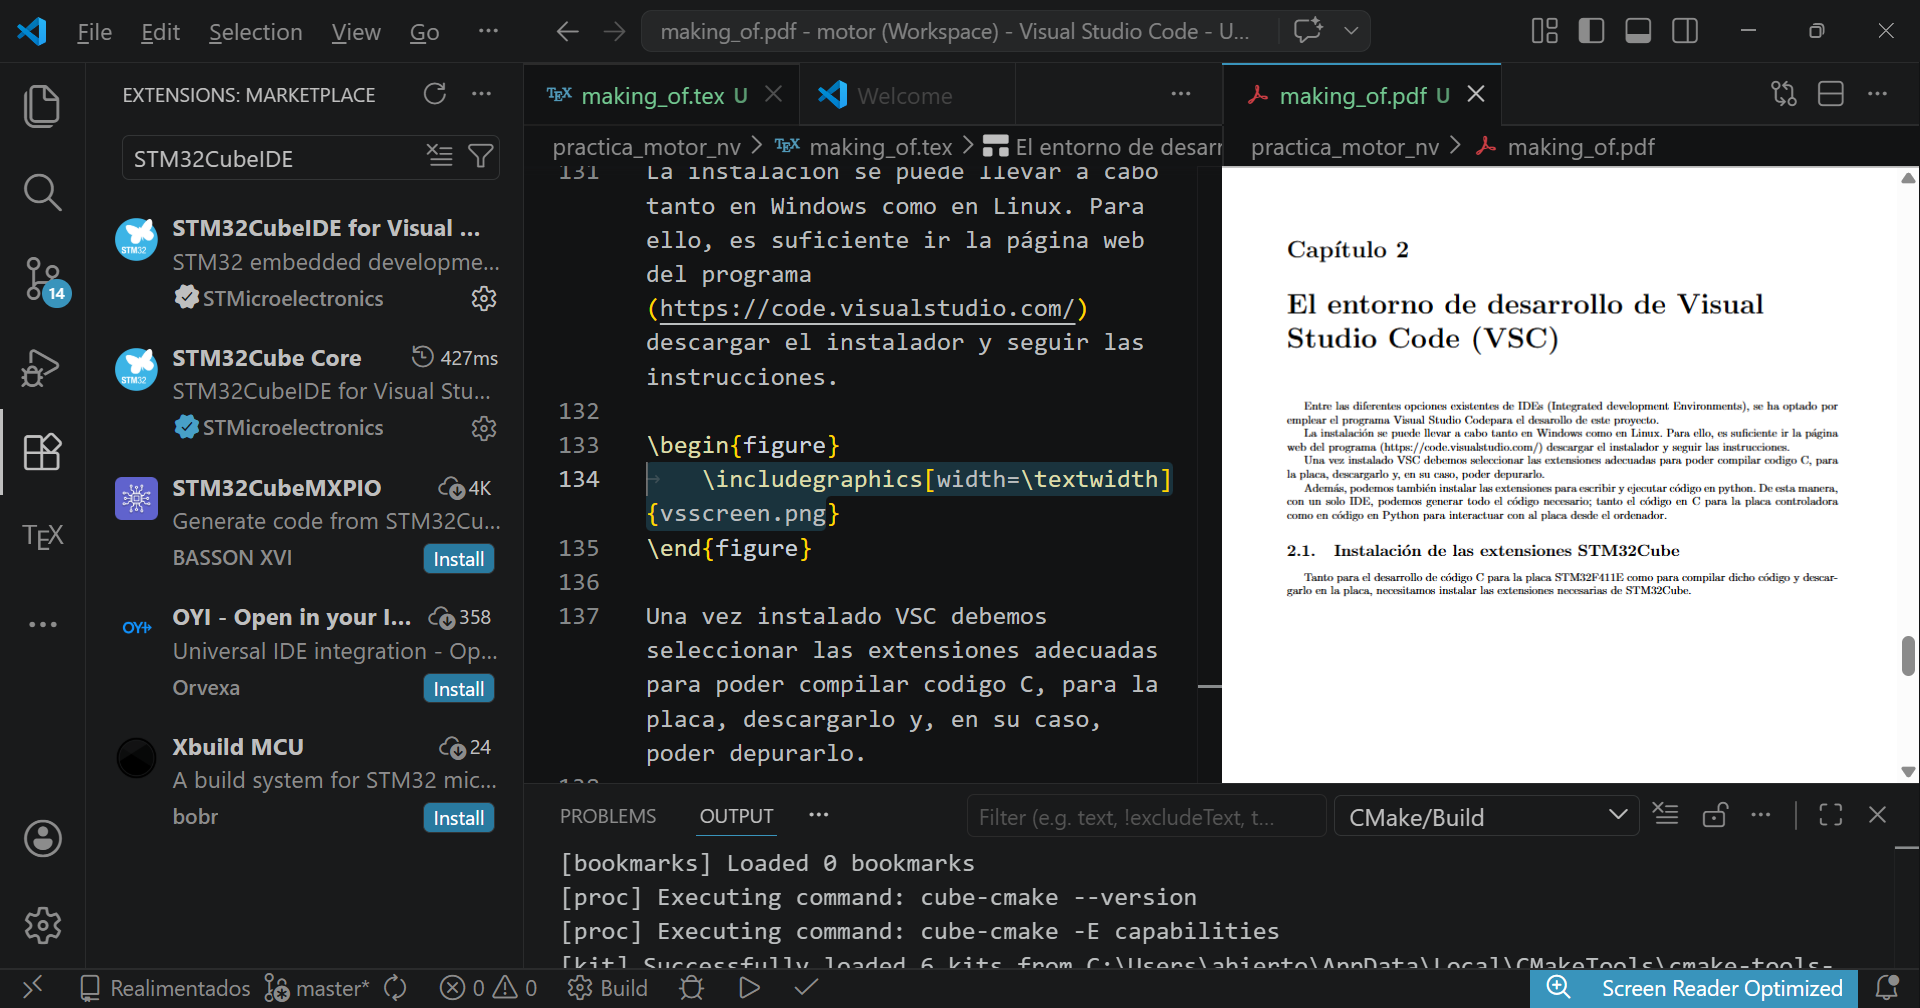
\includegraphics[width=\textwidth]{vsscreen.png}
	\caption{Ventana de Visual Studio Code} \label{fig:vscr}
\end{figure}

Si abrimos el programa, una vez instalado, accedemos a una ventana como la se muestra en la figura \ref{fig:vscr}. Vamos a describir brevemente los elementos más importantes.

\begin{itemize}
	\item Barra de actividad: Es la barra vertical localizada a la izquierda del todo de la ventana. Esta barra permite cambiar la vista del panel situado inmediatamente a su derecha. Las distinta opciones hacen referencias a tareas distintas realizables desde VSC. Así el icono superior (Explorer nos permite navegar por los directorios que tenemos abierto, seleccionar archivos para abrirlos en el editor etc. Debajo tenemos una opción de búqueda (Search). Un control de cambios basado en git (Source control). Un botón para ejecución y depuración de código (RUN and debug), Un botón muy útil que nos permite explorar las extensiones (Extensions) disponibles, es decir configuraciones específicas para manejar distintos tipos de lenguajes de programación, etc.
	\item Barra Lateral, inmediatamente a la derecha de la anterior, ofrece distintas vistas y paneles, dependiendo de la actividad seleccionada en la barra de actividad. En la figura \ref{fig:vscr}, se ve el panel correspondiente a las extensiones, porque la actividad seleccionada, ha sido precisamente el botón extensions. Se pueden recorrer las extensiones disponibles, comprobar si están o no instaladas, y seleccionarla para su instalación/desinstalación, configuración, etc.
	\item El editor. Ocupa el area central. Su objetivo es escribir y editar código. Es posible abrir varios editores uno al lado del otro y de este modo trabajar en varios archivos simultáneamente. En la figura \ref{fig:vscr}, se muestra un fichero de texto que contiene la fuente el \LaTeX con la que se han elaborado estas notas. A su derecha, se ve el texto resultante en un archivo pdf.
	\item Barra de estado (Status Bar) Situada en la parte inferior de la ventana, ofrece información contextual relacionada con el estado actual de VSC y la actividad que se está llevando a cabo.
	\item Paleta de Comandos (Command Palette) Se accede pulsando los comandos Ctrl + Shift + P, es muy útil porque permite el acceso rápido a muchos comandos y características de VSC, sin tener que navegar por menús de opciones.
\end{itemize}

Panels: Panels are located at the bottom of the editor area and can display various tools like the Terminal, Output, Debug Console, and Problems panel.

Tabs: Tabs at the top of the editor allow you to switch between open files quickly. You can also drag and drop tabs to reorder them or open them in new editor groups.

Una vez instalado VSC debemos seleccionar las extensiones adecuadas para poder compilar codigo C, para la placa, descargarlo y, en su caso, poder depurarlo.

Además, podemos también instalar las extensiones para escribir y ejecutar código en python. De esta manera, con un solo IDE, podemos generar todo el código necesario; tanto el código en C para la placa controladora como en código en Python para interactuar con al placa desde el ordenador.

\section{Instalación de las extensiones STM32Cube}
Tanto para el desarrollo de código C para la placa STM32F411E como para compilar dicho código y descargarlo en la placa, necesitamos instalar las extensiones necesarias de STM32Cube.

\end{document}